

\section{GRU vs. Transformer}
It is important here to compare the GRU chatbot with the larger Transformer based chatbot. Using our subjective qualifications the GRU model answers with more variety than the Transformer model. The important observation is that the hyper-parameter set for the Transformer model can be expanded and enlarged as needed before training. The GRU model cannot be trained successfully with an arbitrarily large hyper-parameter set. A larger Transformer can be trained, the benefit associated with this, better responses.

Another observation is that the GRU model responds very quickly, while a Transformer model may take more time relatively. This is not a problem for general applications, but one cannot ignore the time spent by the Transformer model when it is installed on a small computer like a Raspberry Pi. 

The respective value of each of the models changes slightly when you consider what platform they will be implemented on. The GRU responds more quickly and so it retains some worth.

Time complexity is discussed on Youtube by Kaiser et al \cite{youtubeKaiser2017}. For the GRU Recurrent Neural Network it is $ n \cdot d^2 $, where $ n $ is the number of words in a sentence and $ d $ is the dimension of the hidden vector. Complexity for the Transformer's Scaled Dot Product Attention is $ n^2 \cdot  d $. Again, $n$ is the number of words and $d$ is the hidden vector's dimension. 

The maximum allowable input from the GRU is short, and in our example is 10. The maximum allowable input from the Transformer models varies, but in the 117M GPT2 model it is 768. In the Transformer from Section \ref{transformer-movie-corpus} it might be 512. This is the same as the hidden vector size for the Transformer in question.

The hidden vector size for the GRU model is 500 in this example.

\section{Turing Test}

The Turing Test concerns itself with the question of weather a computer is intelligent. Turing says that intelligence is too hard to describe, and that if the computer can convince you that it is intelligent then it is.

Weather this is right is beyond the scope of this paper. The people who trained the Generative Pre-Training 2 transformer were apprehensive about their model's ability to generate human speech. They felt the model worked too well. At first when they finished their model they decided not to release the largest version to the public for several months (Radford et al) \cite{radford2019language}. Ultimately they did release their large model.

The creators of the model used it differently than our chatbot implementation. They generated paragraphs of text, and it was determined at first that the ability of the model to impersonate a human was too great. It was felt that the model could be used to spam facebook and other social networking sites with content that was very convincing. If the model could be used to convince people to act badly, then it should not be released. Humans are susceptible to the sentiments of those they see as their peers. If the model was, for better or worse, passing the Turing test, then it should not fall into the wrong hands. This was the concern of the coders at the time.

Ultimately the large model was released, either because the developers decided the model was not as good as originally estimated, or because they didn't care. 

\section{Word and Sentence Comparisons}

It is important to try to make sense of what is going on in the models during training and inference. In this section there are several graphs and a discussion of the GRU model and the Transformer model and their word and sentence usage.

In these discussions the fully trained GRU and Transformer models are used. They are setup in inference mode and their output is observed when they are exposed to the first 2000 training question sentences from the Movie Subtitles corpus.

\subsection{Word Usage}

In general the Transformer model uses only a small subset of words that it has available to it. In the example below 10,000 input lines were tested from the training set and only a small percentage of the vocabulary words are used by the models in the output. These sentences came from the movie dialog corpus. Some percentage of words are used repeatedly.

\begin{figure}[H]
	\begin{center}
		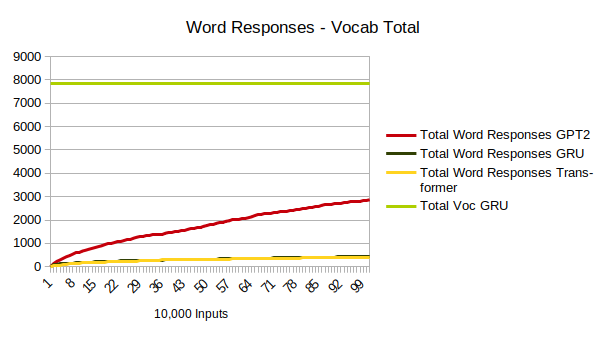
\includegraphics[scale=0.75]{diagram-output-total-responses-01}
		
		
	\end{center}
	\caption[Word Usage]{Word Usage - Including Vocabulary Total}
	
	
\end{figure}

The green line at the top of the graph is the total words in the GRU vocabulary. The total words in the GPT2 vocabulary is not represented on the graph. Total responses in words are shown with the three remaining lines. The GPT2 responses are higher, and the GRU and Transformer responses look like horizontal lines at the bottom of the graph.

If the Vocabulary Total and the GPT2 responses are removed from the diagram the GRU output and the Transformer output take the shape of a curve with a limit somewhere below 475 words. The Transformer model has a vocabulary size of 8170 tokens. The GRU model is close to that at 7826 tokens. Both models use the same training corpus. The difference between the tokens available and the tokens used is large.


\begin{figure}[H]
	\begin{center}
		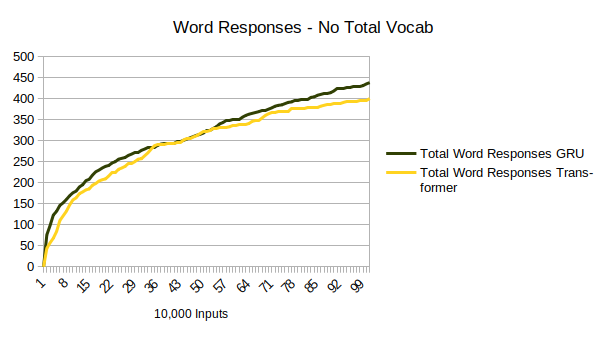
\includegraphics[scale=0.75]{diagram-output-total-responses-02}
		
		
	\end{center}
	\caption[Total Word Responses]{Total Word Responses - No Vocabulary Total}
	
	
\end{figure}

It is possible the GRU model operates more robustly than the Transformer model, or the Transformer model may be over trained or over fitted. It also might be that the hyper parameter set is poorly adjusted. The learning rate, for example, may be too high.

\subsection{Sentence Usage}

How many fully formed responses does the given model use? Additionally when or how many of these responses are used repeatedly?

The GPT2 model is very large and very versatile, but the Transformer model and the GRU model are smaller. For these two smaller models it would be good to tell how many repeated sentences occurred as output in some number of inputs. For the graph 10,000 inputs from the training set of the movie dialog corpus are used. % in contrast to the previous section where 2000 inputs are used.

There are rough numbers for those two models. They use about 350 sentences repeatedly. As for total sentences used the GRU is increasing still at 900 sentences at the end of our study. It is assumed at some point the number of total GRU sentences that that model can produce reaches some kind of limit.

\begin{figure}[H]
	\begin{center}
		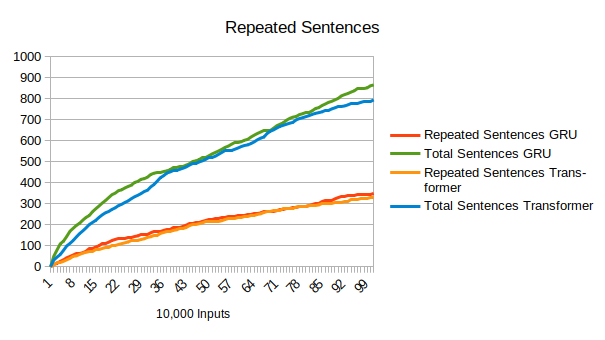
\includegraphics[scale=0.75]{diagram-output-repeated}
		
		
	\end{center}
	\caption[Simple Sentence Usage]{Simple Sentence Usage}
	
	
\end{figure}


The interesting thing is that the Transformer and the GRU models both have similar `Repeated Sentence' graphs. They are totally different models and have totally different sizes. They are not similar in many ways but in this metric. They share the same corpus, so they may be learning the same task.

\section{Training and Lists}
In this discussion the output of the GPT2 model is mostly ignored. %There is a short discussion of the Transformer and the GRU.

What is the Transformer or GRU doing during training and later during inference. Here the Transformer and GRU models are trained on the movie dialog corpus. The Transformer model in question has 6 layers, 8 heads, and a hidden size of 512 units. The GRU model has a hidden size of 500.

It seems the model learns a set of multi-purpose English answers in a form close to a list. Then it spends time as a classifier. Each input sentence is compared to the set of answers. A question is associated with a given answer from the set when possible. There would be fewer answers than there are questions. It is as if there were a list somewhere that contained many of the answers that the model would use. For a given model this list can only be so long.

It is interesting to point out that probably at the start the multi-purpose answers are constructed at the same time that the classification task is taking place. 

This list making is a function of the model trying to optimize the answers that it gives, and can give, given a certain size memory capacity. The model has a certain capacity and it starts to develop lists of usable answers in order to use that capacity best.

For the very large pre-trained model, like the GPT2, full sentences may not be saved. These models may be more dynamic. For translation for instance, the same model may be able to remember longer lists, or in place of a list of complete responses keep a list of phrases or partial responses that could be combined to create translated output.

The output of the Transformer or GRU, shows little intelligence. The actual utterances of the model are pretty plain. The internal building of lists, though, shows a process that is found in some intelligent activity.